\documentclass{article}
\usepackage{amsmath}
\usepackage{amssymb}
\usepackage{graphicx}
\usepackage{hyperref}
\usepackage[version=4]{mhchem}


\begin{document}
\(\triangle A B C\) is a right isosceles triangle with \(\angle A C B=90^{\circ}\) and \(A C=B C\).\\
\centering
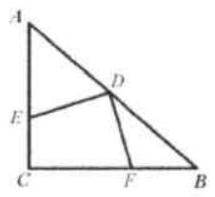
\includegraphics[width=\textwidth]{images/012(3).jpg}

Point \(D\) is the midpoints on sides \(A B . D E \perp D F\). Points \(E, F\) are on sides \(A C\) and \(B C\), respectively. Show that \(D E=D F\).

Solution:
Draw \(C D\), the median of triangle \(A B C\). Since \(C D\) is the median, by Theorem 1.3, \(C D=A D=B D\).\\
\(\angle A C D=45^{\circ} . \angle B=45^{\circ}\).\\
\(\angle B D F+\angle F D C=90^{\circ}\).\\
\(\angle F D C+\angle C D E=90^{\circ}\).\\
\(\angle B D F=\angle C D E=\alpha\).\\
\(\angle A C D=\angle E C D=\angle B=45^{\circ}\).\\
\centering
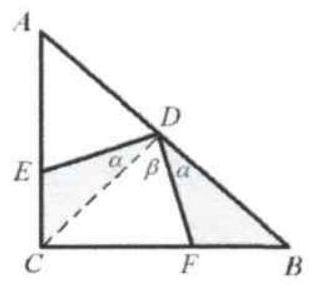
\includegraphics[width=\textwidth]{images/013.jpg}\\
\(\triangle C E D \cong \triangle B F D\).\\
Thus \(D E=D F\).


\end{document}
